\documentclass[12pt,a4paper]{article}
\usepackage[MeX]{polski}
\usepackage[utf8]{inputenc}
\usepackage{listings}
\usepackage{graphicx}
\usepackage{fancyvrb}
\usepackage{tabularx}
\usepackage{geometry}
\usepackage{multirow}
\usepackage{amsmath}
\usepackage[hidelinks]{hyperref}
\geometry{
 a4paper,
 total={170mm,257mm},
 left=20mm,
 top=20mm,
}
\author{Yurii~Vyzhha}
\title{Metody Obliczeniowe w Nauce i Technice \\ Laboratorium 1 \\
  Arytmetyka Komputerowa \\ Sprawozdanie}
\begin{document}
  \maketitle
  \paragraph{Zadanie 1 Metoda Gaussa-Jordana}
  \begin{Verbatim}
      function b = GaussJordan(A, b)
          [n,~] = size(A);
          for k = 1:n
              for i = k+1:n
                  xmult = A(i,k)/A(k,k);
                  for j = k+1:n
                      A(i,j) = A(i,j) - xmult*A(k,j);
                  end
                  b(i) = b(i) - xmult*b(k);
              end
              for i = k-1:-1:1
                  xmult = A(i,k)/A(k,k);
                  for j = k+1:n
                      A(i,j) = A(i,j) - xmult*A(k,j);
                  end
                  b(i) = b(i) - xmult*b(k);
              end
          end
          for k = 1:n
              b(k) = b(k)/A(k,k);
          end
      end
  \end{Verbatim}
  Metoda ta działa w podobny sposób do zwykłej metody Gaussa. Różni się głównie
  tym, że w algorytmie Gaussa-Jordana eliminujemy elementy nie tylko "idąc w dół",
  a i "idąć w górę". Inną cechą też jest dzielenie elementów $b_i$ przez
  odpowiednie im elementy $A_{ii}$, gdzie $1 \leq i \leq n$.\newline
  Dla sprawdzenia poprawności tej funkcji używam następującej funkcji:
  \begin{Verbatim}
      function a = CheckGaussJordan(A,b)
          x = GaussJordan(A,b);
          [~,n] = size(x);
          a = true;
          for i = 1:n
              sum = 0;
              for j = 1:n
                  sum = sum + A(i,j)*x(j);
              end
              if abs(sum - b(i)) > 1e12*eps(min(abs(sum),abs(b(i))))
                  disp(sum);
                  disp(b(i));
                  a = false;
                  break
              end
          end
      end
  \end{Verbatim}
Funkcja ta podstawia znalezione pierwiastki do równań i sprawdza czy nie ma
sprzeczności.\newline
Następną częścią tego zadania było porównanie szybkości działania napisanej
oraz bibliotecznej funkcji dla macierzy rozmiaru $500 \times 500$. Niżej podaję
wyniki dla pięciu różnych losowych macierzy:\newline
\begin{tabularx}{\textwidth}{ l l }
    Moja & Biblioteczna \\
    0.805022 & 3.717958 \\
    0.724206 & 3.734668 \\
    0.717710 & 3.695297 \\
    0.703726 & 3.708560 \\
    0.690628 & 3.735460 \\
\end{tabularx}\vspace{3mm}\newline
To, że biblioteczna funkcja działa wolniej od napisanej przeze mnie można
wyjaśnić tym faktem, że ta pierwsza prawdopodobnie sprawdza rozmiary macierzy,
czy tą macierz da się obliczyć etc., czego nie robi moja funkcja.
  \paragraph{Zadanie 2 Faktoryzacja LU}%\mbox{}\vspace{3mm}\\
  \begin{Verbatim}
    function [p, A] = LU(A)
        [n,~] = size(A);
        s = zeros(1,n);
        p = zeros(1,n);
        for i = 1:n
            s(i) = max(abs(A(i,:)));
            p(i) = i;
        end
        for k = 1:n-1
            rmax = 0;
            for i = k+1:n
                r = abs(A(i,k)/s(i));
                if r > rmax
                    rmax = r;
                    imax = i;
                end
            end
            if k ~= imax
                tmp = P(k);
                p(k) = p(imax);
                p(imax) = tmp;
                A([k imax],:) = A([imax k],:);
            end
            for i = k+1:n
                xmult = A(i,k)/A(k,k);
                A(i,k) = xmult;
                for j = k+1:n
                    A(i,j) = A(i,j) - xmult*A(k,j);
                end
            end
        end
    end
  \end{Verbatim}
  Funkcja działa w następujący sposób. Najpierw tworzymy dwa wektory: $s$ oraz $p$.
  $s$ jest wektorem skalowania takim, że
  $s_i = \underset{1 \leq j \leq n}{\mathrm{max}}\lvert A_{ij} \rvert$.
  $p$ jest wektorem reprezentującym macierz zamiany rzędów $P$. Tą macierz można otrzymać
  najpierw tworząc macierz zerową $n \times n$ oraz w miejscach tej macierzy $(i,p(i))$
  wpisać jedynki. W głównej pętli $1 \leq k \leq n-1$, gdzie $n$ to rozmiar macierzy A,
  szukamy elementu $rmax$ takiego, że
  $\mathrm{rmax} = \underset{k+1 \leq i \leq n}{\mathrm{max}} \lvert \frac{A_{ik}}{s_i} \rvert$.
  W danej interacji pętli, rmax jest pivotem, a imax jest indexem rzędu, w
  którym go znaleźliśmy. Jeśli $\mathrm{imax} \neq \mathrm{k}$ to zamieniamy
  rzędy miejscami, zapisując zmiany w vector $P$. Następnie w pętlin $i = k+1:n$ obliczamy
  współczynnik xmult, za pomocą którego redukujemy rzędy od $k+1$ do $n$. Ten współczynnik
  wpisujemy na miejśce $A_{ik}$; on będzie elementem macierzy $L$. Po wykonianiu się
  programu dostajemy na wyjściu wektor P oraz macierz zmienioną macierz $A$, w
  której są jednocześnie zapisane macierze $L$ oraz $U$. \newline
  Dla sprawdzenia poprawności danej funkcji, napisałem program, który sprawdza, czy
  dla $P$, $L$ i $U$, otrzymanych jako wyniki funkcji faktoryzującej, zachodzi
  $P*A=L*U$.
\begin{Verbatim}
    function a = CheckLU(A)
        [n,~] = size(A);
        [p, lu] = LU(A);
        P = zeros(n);
        for i = 1:n
            P(i,p(i)) = 1;
        end
        L = eye(n);
        U = zeros(n);
        for i = n:-1:1
            for j = n:-1:i
                U(n-j+1,n-i+1) = lu(n-j+1,n-i+1);
            end
        end
        for i = 2:n
            for j = 1:i-1
                L(i,j) = lu(i,j);
            end
        end
        X = P*A;
        Y = L*U;
        a = true;
        for i = 1:n
            for j = 1:n
                if abs(X(i,j)-Y(i,j)) > 1e12*eps(min(abs(X(i,j)),abs(Y(i,j))))
                    a = false;
                    break
                end
            end
        end
    end
\end{Verbatim}
W tej funkcji oblicamy $P$, $L$ i $U$ za pomocą wspomnianej wyżej funkcji oraz
tworzymy nowe macierze $X=P*A$ i $Y=L*U$. Dalej porównujemy każdy odpowiedni element
macierzy $X$ oraz $Y$ i zwracamy "prawdę", jeśli $X_{ij}$ jest prawie równe
$Y_{ij}$ dla każdego $1 \leq i \leq n$ oraz $1 \leq j \leq n$.
\paragraph{Zadanie 3 Analiza obwodu elektrycznego}\mbox{}\vspace{3mm}\\
Działanie programu, który rozwiązuję dane zadanie, krótko można opisać w
następujący sposób:
\begin{enumerate}
    \item Wczytaj z pliku wierzchołki i krawędzi i stwróż z nich graf opisujący
    obwód elektrycny.
    \item Znajdź wszystkie cykle w grafie.
    \item Załóż kierunek przepływu prądu sprowadając wygenerowane cylke do
    postaci skierowanej.
    \item Posortuj te cykle według ich długości.
    \item Zostaw tylko te cykle, które zawierają nowe krawędzie.
    \item Dla każdej krawędzi zapamiętaj cyklę, które przechodzą przez nią.
    \item Stwórz macierz $A$ uwzględniając wszyskie prądy płynące przez każdy
    obwód (cykl) oraz wektor $b$ uwzględniając wszystkie źródła napięcia w obwodzie.
    \item Rozwiąż układ $A*b = x$. W wektorze $x$ mamy prądy, które płyną w obwodach.
    \item Policz napięcie na każdej krawędzi, uwzględniając wszyskie prądy
    płynące przez tą krawędź. Jeśli napięcie jest ujemne, odwróć jej kierunek.
    \item Narysuj wczytany graf dopisując wartości napięć na krawędziach.
\end{enumerate}
Niżej podaję pokrokowe rozwiązanie problemu wraz z kodem.
\subparagraph{1.} Definicja grafu, wierzchołków i krawędzi.
\begin{Verbatim}[fontsize=\small]
    public class Vertex {
    	private int id;

    	Vertex(int id) {
    	    this.id = id;
        }

    	int getId() {
    	    return this.id;
        }

    	@Override
    	public String toString() {
    		return "(" + id + ")";
    	}

    	@Override
    	public int hashCode() {
    		final int prime = 31;
    		int result = 1;
    		result = prime * result + id;
    		return result;
    	}

    	@Override
    	public boolean equals(Object obj) {
    		if (this == obj)
    			return true;
    		if (obj == null)
    			return false;
    		if (getClass() != obj.getClass())
    			return false;
    		Vertex other = (Vertex) obj;
    		return id == other.id;
    	}
    }
\end{Verbatim}
Każdy wierzchołek ma unikalne id, stąd przyjąłem że dwa wierzchołki są sobie
równe jeżeli ich id są równe.
\begin{Verbatim}[fontsize=\small]
    public class Edge {
        private final Vertex source;
        private final Vertex destination;
        private double weight;
        private boolean isVoltage;
        private int voltageDirection;

        public Edge(Vertex source, Vertex destination) {
            this.source = source;
            this.destination = destination;
            this.weight = 0.0;
            this.isVoltage = false;
            this.voltageDirection = 0; // - -> + == > 0; + -> - == < 0
        }

        public Edge(Vertex source, Vertex destination, double weight) {
            this.source = source;
            this.destination = destination;
            this.weight = weight;
            this.isVoltage = false;
            this.voltageDirection = 0;
        }

        int getVoltageDirection() {
            return voltageDirection;
        }

        void setVoltageDirection(int voltageDirection) {
            this.voltageDirection = voltageDirection;
        }

        public Vertex getDestination() {
            return destination;
        }

        public Vertex getSource() {
            return source;
        }

        public double getWeight() {
            return weight;
        }

        public boolean isVoltage() {
            return isVoltage;
        }

        void setVoltage() {
    	    isVoltage = true;
        }

        @Override
        public String toString() {
            return source + "-" + destination;
        }

        @Override
        public int hashCode() {
            int x = source.getId();
            int y = destination.getId();
            return ((x + y)*(x + y + 1))/2 + y;
        }

        @Override
        public boolean equals(Object obj) {
            if (this == obj)
    	    return true;
    	if (obj == null)
    	    return false;
    	if (getClass() != obj.getClass())
    	    return false;
    	Edge other = (Edge) obj;
    	if (destination == null) {
    	    if (other.destination != null)
                    return false;
            } else if (!destination.equals(other.destination))
                return false;
            if (source == null) {
                if (other.source != null)
                    return false;
            } else if (!source.equals(other.source))
                return false;
    	return true;
        }

    }
\end{Verbatim}
Pole isVoltage mówi o tym, czy na krawędzi znajduje się źródło napięcia czy
rezystor. Jeśli na krawędzi znajduje się źródło napięcia, to voltageDirection
wskazuje kierunek napięcia. \newline
Jako funkcję hashującą wybrałem funkcję pary Kantora. \newline
Klasa odpowiedalna za wczytywanie grafu:
\begin{Verbatim}[fontsize=\small]
    public class GraphReader {
        private File file;
        private MyGraph graph;

        public GraphReader(File file) {
            this.file = file;
            graph = new MyGraph();
        }

        public void readFromFile() throws FileNotFoundException {
            Scanner scanner = new Scanner(new FileInputStream(file));
            boolean isVoltageEdge = false;
            while (scanner.hasNextLine()) {
                String line = scanner.nextLine();
                if (line.trim().length() == 0) {
                    isVoltageEdge = true;
                    continue;
                }
                String[] data = line.split(" ");
                int vertex1Id = Integer.parseInt(data[0]);
                int vertex2Id = Integer.parseInt(data[1]);
                double weight = Double.parseDouble(data[2]);
                if(isVoltageEdge) {
                    graph.addBidirectionalVoltageEdge(vertex1Id, vertex2Id, weight);
                } else {
                    graph.addBidirectionalEdge(vertex1Id, vertex2Id, weight);
                }
            }
        }

        public MyGraph getGraph() {
            return graph;
        }
    }
\end{Verbatim}
Mój program pozwala na wczytanie więcej niż jednego źródła napięcia.
\subparagraph{2} Dla znalezienia wszystkich cyklów wykorzystałem klasę \emph{CycleUtil}
napisaną przez \newline \mbox{\emph{lucaslouca}}, znajdująca się pod adresem:
\url{https://github.com/lucaslouca/graph-cycles}. \newline Metoda \mbox{\emph{listAllCycles()}} zwraca
listę cykli jako listę grafów nieskierowanych.
\subparagraph{3} Klasa CycleTransform jest odpowiedzialna za sprowadzanie cylki
do postaci, z której możemy już wczytać informacje do macierzy.
\begin{Verbatim}[fontsize=\small]
    public class CycleTransform {
        private List<MyGraph> cyclesAsGraphList;

        public CycleTransform(List<MyGraph> cyclesList) {
            this.cyclesAsGraphList = cyclesList;
        }

        public List<List<Edge>> getCyclesFromGraphs() {
            List<List<Edge>> cycles = new ArrayList<>();
            for(MyGraph g : cyclesAsGraphList) {
                cycles.add(g.getEdges());
            }
            return cycles;
        }

        public List<List<Edge>> removeRedundantEdges(List<List<Edge>> rawCycles) {
            int currentSourceId;
            int currentDestinationId;
            List<List<Edge>> resultCycles = new ArrayList<>();
            for (int i = 0; i < rawCycles.size(); i++) {
                List<Edge> currentRawCycle = rawCycles.get(i);
                resultCycles.add(new ArrayList<>());
                List<Edge> currentResultCycle = resultCycles.get(i);
                currentSourceId = currentRawCycle.get(0).getSource().getId();
                currentDestinationId = currentRawCycle.get(0).getDestination().getId();
                int loopInv = currentRawCycle.size() / 2;

                for (int k = 0; k < loopInv; k++) {
                    for (int j = 0; j < currentRawCycle.size(); j++) {
                        if(currentRawCycle.get(j).getSource().getId() == currentSourceId &&
                                currentRawCycle.get(j).getDestination().getId() == currentDestinationId) {
                            currentResultCycle.add(currentRawCycle.remove(j));
                            break;
                        }
                    }
                    for (int j = 0; j < currentRawCycle.size(); j++) {
                        if(currentRawCycle.get(j).getDestination().getId() == currentSourceId &&
                                currentRawCycle.get(j).getSource().getId() == currentDestinationId) {
                            currentRawCycle.remove(j);
                            break;
                        }
                    }
                    for (Edge aCurrentRawCycle : currentRawCycle) {
                        if (aCurrentRawCycle.getSource().getId() == currentDestinationId) {
                            currentSourceId = aCurrentRawCycle.getSource().getId();
                            currentDestinationId = aCurrentRawCycle.getDestination().getId();
                            break;
                        }
                    }
                }
            }
            return resultCycles;
        }

        public void sortCyclesByLength(List<List<Edge>> cycles) {
            cycles.sort((l1, l2) -> (l1.size() - l2.size()));
        }

        public void removeRedundantCycles(List<List<Edge>> cycles) {
            Set<Edge> appearedEdgesSet = new HashSet<>();
            boolean foundNewEdge = false;
            for (int i = 0; i < cycles.size(); i++) {
                for (Edge e : cycles.get(i)) {
                    if(isNewEdge(appearedEdgesSet, e)) {
                        appearedEdgesSet.add(e);
                        foundNewEdge = true;
                    }
                }
                if(!foundNewEdge) {
                    cycles.remove(i);
                    i--;
                }
                foundNewEdge = false;
            }
        }

        boolean isNewEdge(Set<Edge> appearedEdgesSet, Edge e) {
            return !(appearedEdgesSet.contains(e) ||
                    appearedEdgesSet.contains(new Edge(e.getDestination(), e.getSource())));
        }

    }
\end{Verbatim}
Metoda \emph{removeRedundantEdges()} usuwa powtarzające się krawędzie oraz ustawia ich
w kierunku, który wybieramy losowo. Ta losowość nie ma wpływu na poprawność
działania programu, musimy poprostu zapamiętać kierunek dla tego cyklu względem
innych.
\subparagraph{4} Metoda \emph{sortCyclesByLength()} sortuje krawędzi według długości. Robimy to
dla tego, żeby zostawić tylko najkrótsze cykle z tych, które nam potrzebne. To
trochę przyspiesza działanie programu.
\subparagraph{5} Metoda \emph{removeRedundantCycles()} przechodzi po wszyskich cyklach i zapamiętuję
napotkane krawędzie. Jeśli w kolejnej iteracji pętli programu napotkaliśmy cykl,
który zawiera wyłącznie już napotkane krawędzie to usuwamy go. W taki sposób
pozbawiamy się nadmiarowości przy tworzeniu macierzy.
\subparagraph{6} Tworzeniem i wypełnianiem macierzy $A$ oraz wektora $b$ zajmuje
się klasa \emph{MatrixPreparer}.
\begin{Verbatim}[fontsize=\small]
    public class MatrixPreparer {
        private List<List<Edge>> cycles;
        private double[][] matrix;
        private double[][] vector;
        private LinkedHashMap<Edge, List<CurrentDirection>> edgeCurrentsMap;

        public MatrixPreparer(List<List<Edge>> cycles) {
            this.cycles = cycles;
            int n = cycles.size();
            matrix = new double[n][n];
            vector = new double[n][n];
            for (int i = 0; i < matrix.length; i++) {
                for (int j = 0; j < matrix[i].length; j++) {
                    matrix[i][j] = 0.0;
                }
                vector[i][0] = 0.0;
            }
            edgeCurrentsMap = new LinkedHashMap<>();
        }

        public void fillMap() {
            for (int i = 0; i < cycles.size(); i++) {
                List<Edge> cycle = cycles.get(i);
                for (Edge edge : cycle) {
                    if (!edgeCurrentsMap.containsKey(edge)) {
                        List<CurrentDirection> currentDirections = new ArrayList<>();
                        currentDirections.add(new CurrentDirection(i, edge.getWeight()));
                        edgeCurrentsMap.put(edge, currentDirections);
                    } else {
                        edgeCurrentsMap.get(edge).add(new CurrentDirection(i, edge.getWeight()));
                    }

                }
            }
        }

        public void fillMatrix() {
            for (int i = 0; i < cycles.size(); i++) {
                fillRow(i);
            }
        }

        void fillRow(int i) {
            List<Edge> currentRow = cycles.get(i);
            for (Edge currentEdge : currentRow) {
                if (currentEdge.isVoltage()) {
                    if (currentEdge.getVoltageDirection() < 0) {
                        vector[i][0] = currentEdge.getWeight();
                    } else {
                        vector[i][0] = -currentEdge.getWeight();
                    }
                } else {
                    if (currentEdge.getWeight() != 0.0) {
                        matrix[i][i] += currentEdge.getWeight();
                        checkInfoAboutEdge(i, currentEdge);
                    }
                }
            }
        }

        void checkInfoAboutEdge(int i, Edge currentEdge) {
            Edge reversedEdge = new Edge(
                    currentEdge.getDestination(),
                    currentEdge.getSource(),
                    currentEdge.getWeight()
            );
            List<CurrentDirection> currents;
            if (edgeCurrentsMap.containsKey(currentEdge)) {
                currents = edgeCurrentsMap.get(currentEdge);
                for (CurrentDirection current : currents) {
                    int j = current.getCurrentNum();
                    if (i != j) {
                        matrix[i][j] += current.getWeight();
                    }
                }
            }
            if (edgeCurrentsMap.containsKey(reversedEdge)) {
                currents = edgeCurrentsMap.get(reversedEdge);
                for (CurrentDirection current : currents) {
                    int j = current.getCurrentNum();
                    if (i != j) {
                        matrix[i][j] -= current.getWeight();
                    }
                }
            }
        }

        public LinkedHashMap<Edge, List<CurrentDirection>> getEdgeCurrentsMap() {
            return edgeCurrentsMap;
        }

        public double[][] getMatrix() {
            return matrix;
        }

        public double[][] getVector() {
            return vector;
        }
    }
\end{Verbatim}
\emph{fillMap()} zapamiętuje numery cyklów dla każdego wierzchołka. Przechowywanie
numerów odbywa się w obiektach klasy \emph{CurrentDirection}.
\begin{Verbatim}[fontsize=\small]
    public class CurrentDirection {
        private int currentNum;
        private double weight;

        CurrentDirection(int c, double w) {
            this.currentNum = c;
            this.weight = w;
        }

        public int getCurrentNum() {
            return currentNum;
        }

        double getWeight() {
            return weight;
        }
    }
\end{Verbatim}
\subparagraph{7} Metoda \emph{fillMatrix()} wypelnia macierz $A$ i wektor $b$
przez wywołanie pomocniczych metod \emph{fillRow()} oraz \emph{checkInfoAboutEdge()}.
\emph{fillRow()} wypełnia pozycję $A_{ii}$ oraz $b_i$, gdzie $0 \leq i < n$.
\emph{checkInfoAboutEdge()} wypełnia pozostałe pozycje.
\subparagraph{8} Dla rozwiązywania otrzymanego układu równań, korzystałem z
metody \emph{solve()} z biblioteki algebry liniowej JAMA.
\begin{Verbatim}[fontsize=\small]
    Matrix a = new Matrix(matrixPreparer.getMatrix());
    Matrix b = new Matrix(matrixPreparer.getVector());
    Matrix x = a.solve(b);
\end{Verbatim}
\subparagraph{9} Dla tworzenia grafu dla wizualizacji stosuję klasę
\emph{VisualGraphMaker}.
\begin{Verbatim}[fontsize=\small]
    public class VisualGraphMaker {
        private Graph<Vertex, Edge> resultGraph;
        private List<Vertex> vertices;
        private Matrix b;
        private LinkedHashMap<Edge, List<CurrentDirection>> edgeCurrentsMap;

        public VisualGraphMaker(
                Matrix b,
                List<Vertex> vertices,
                LinkedHashMap<Edge, List<CurrentDirection>> edgeCurrentsMap
        )
        {
            this.b = b;
            resultGraph = new DirectedSparseGraph<>();
            this.vertices = vertices;
            this.edgeCurrentsMap = edgeCurrentsMap;
        }

        public void createGraph() {
            for (Vertex v : vertices) {
                resultGraph.addVertex(v);
            }
            Set<Edge> visitedEdges = new HashSet<>();
            for (Map.Entry<Edge, List<CurrentDirection>> entry : edgeCurrentsMap.entrySet()) {
                Edge edge = entry.getKey();
                Edge reversedEdge = new Edge(
                        edge.getDestination(),
                        edge.getSource(),
                        edge.getWeight()
                );
                if(!visitedEdges.contains(reversedEdge)) {
                    visitedEdges.add(edge);
                    List<CurrentDirection> directions = entry.getValue();
                    double result = 0.0;
                    if(edge.isVoltage()) {
                        result = edge.getWeight();
                    } else {
                        for (CurrentDirection direction : directions) {
                            int i = direction.getCurrentNum();
                            result += b.get(i, 0);
                        }
                        if(edgeCurrentsMap.containsKey(reversedEdge)) {
                            List<CurrentDirection> otherDirections =
                                edgeCurrentsMap.get(reversedEdge);
                            for (CurrentDirection direction : otherDirections) {
                                int i = direction.getCurrentNum();
                                result -= b.get(i, 0);
                            }
                        }
                        result = result * edge.getWeight();
                    }
                    if (result > 0) {
                        resultGraph.addEdge(
                                new Edge(edge.getSource(), edge.getDestination(), result),
                                edge.getSource(),
                                edge.getDestination()
                        );
                    } else {
                        resultGraph.addEdge(
                                new Edge(edge.getDestination(), edge.getSource(), -result),
                                edge.getDestination(),
                                edge.getSource()
                        );
                    }
                }
            }
        }

        public Graph<Vertex, Edge> getResultGraph() {
            return resultGraph;
        }
    }
\end{Verbatim}
W tej klasie metoda \emph{createGraph()} przechodzi po wszystkich krawędziach,
oblicza sumę wszyskich prądów, przechodzących przez tą krawędź, i tworzy nową
krawędź z wagą równą obliczonej sumie razy rezystancji. Kierunek krawędzi
zależy o tego czy otrzymany wynik jest większy od zera. W taki sposób mamy
możliwość graficznie reprezentować kierunek przepływu prądu.
\subparagraph{10} Dla rysowania grafu korzystam z biblioteki Jung. Wszystkie
sprawy związane z rysowaniem grafu wykonują się w klase \emph{Visualizer}.
\begin{Verbatim}[fontsize=\small]
    public class Visualizer {

        private BasicVisualizationServer<Vertex, Edge> basicVisualizationServer;

        public Visualizer(Graph<Vertex, Edge> graph) {
            Layout<Vertex, Edge> layout = new FRLayout<>(graph);
            this.basicVisualizationServer = new BasicVisualizationServer<>(layout);
        }

        public void setContext() {
            DecimalFormat df = new DecimalFormat("#.##");
            basicVisualizationServer
                    .getRenderContext()
                    .setEdgeLabelTransformer(edge -> df.format(edge.getWeight()));
            basicVisualizationServer
                    .getRenderContext()
                    .setVertexLabelTransformer(Vertex::toString);
            basicVisualizationServer.setPreferredSize(new Dimension(900, 700));
        }

        public void initializeFrame() {
            JFrame frame = new JFrame("graph");
            frame.setDefaultCloseOperation(WindowConstants.EXIT_ON_CLOSE);
            frame.getContentPane().add(basicVisualizationServer);
            frame.pack();
            frame.setLocationRelativeTo(null);
            frame.setVisible(true);
        }
    }
\end{Verbatim}
Niżej przedstawiam przykładowy rysunek grafu.
\begin{center}
    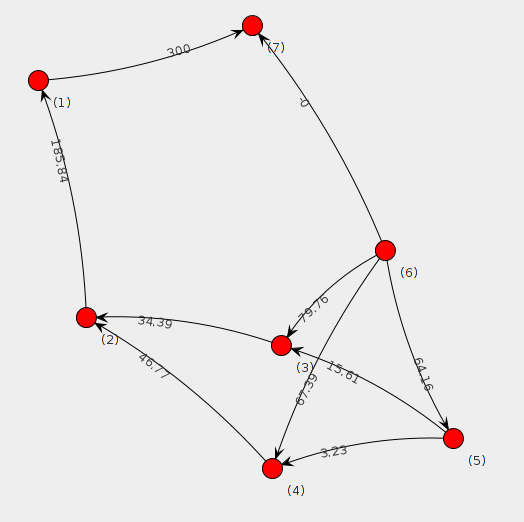
\includegraphics[width=0.8\textwidth]{img/graph}
\end{center}

\end{document}
